\documentclass[../thesis.tex]{subfiles}

\begin{document}

\appendix

\chapter{Data Description}
\label{chap:data_desc}

\noindent In this appendix we present a descriptive overview of the data used in this thesis. This includes: an overview and explanation of the variables used (\ref{sec:variables}), the \texttt{R}-packages (\ref{sec:r_pack}) used and some relevant plots (\ref{sec:rel_plots}) to support the finding in the thesis. The source code used to produce the relevant plots can be found in appendix (\ref{chap:souce_code}).  

\section{Variables}
\label{sec:variables}

\section{\texttt{R}-packages}
\label{sec:r_pack}

\section{Descriptive Statistics}
\label{sec:desc_stat}



\newpage

\section{Relevant Plots}
\label{sec:rel_plots}

\begin{figure}[h!]
    \centering
    \hspace*{-1cm}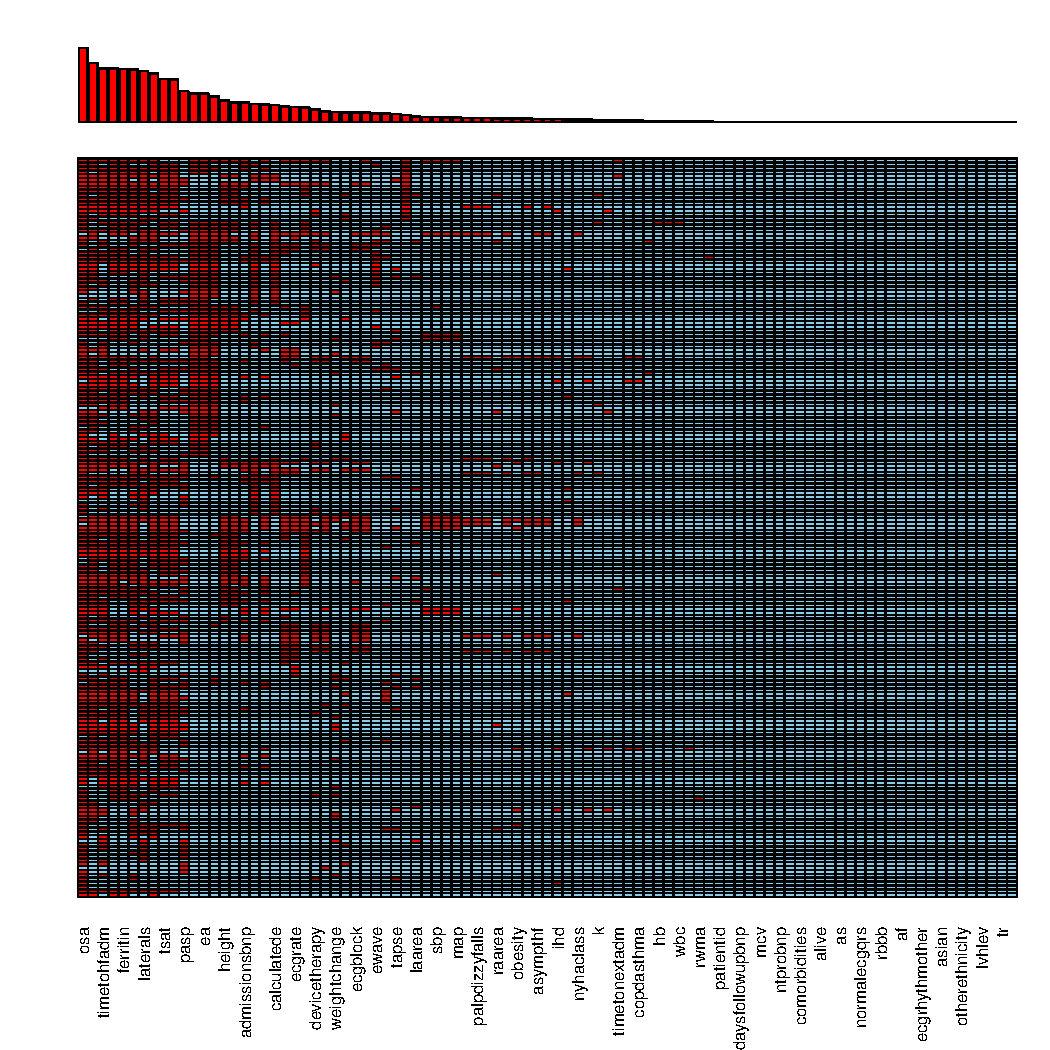
\includegraphics[width=1.1\textwidth]{doc/thesis/images/HFpEF_miss_dist.pdf}
    \caption[Missing values in HFpEF data set]{\textit{Missing values in HFpEF data set. Top:  the amount of missing values in each variable sorted in ascending order. Bottom: plot of the combinations of missing (red) and non-missing (blue) values in the HFpEF data set.}}
    \label{fig:HFpEF_missing}
\end{figure}

\newpage

\begin{figure}[h!]
    \centering
    \hspace*{-1cm}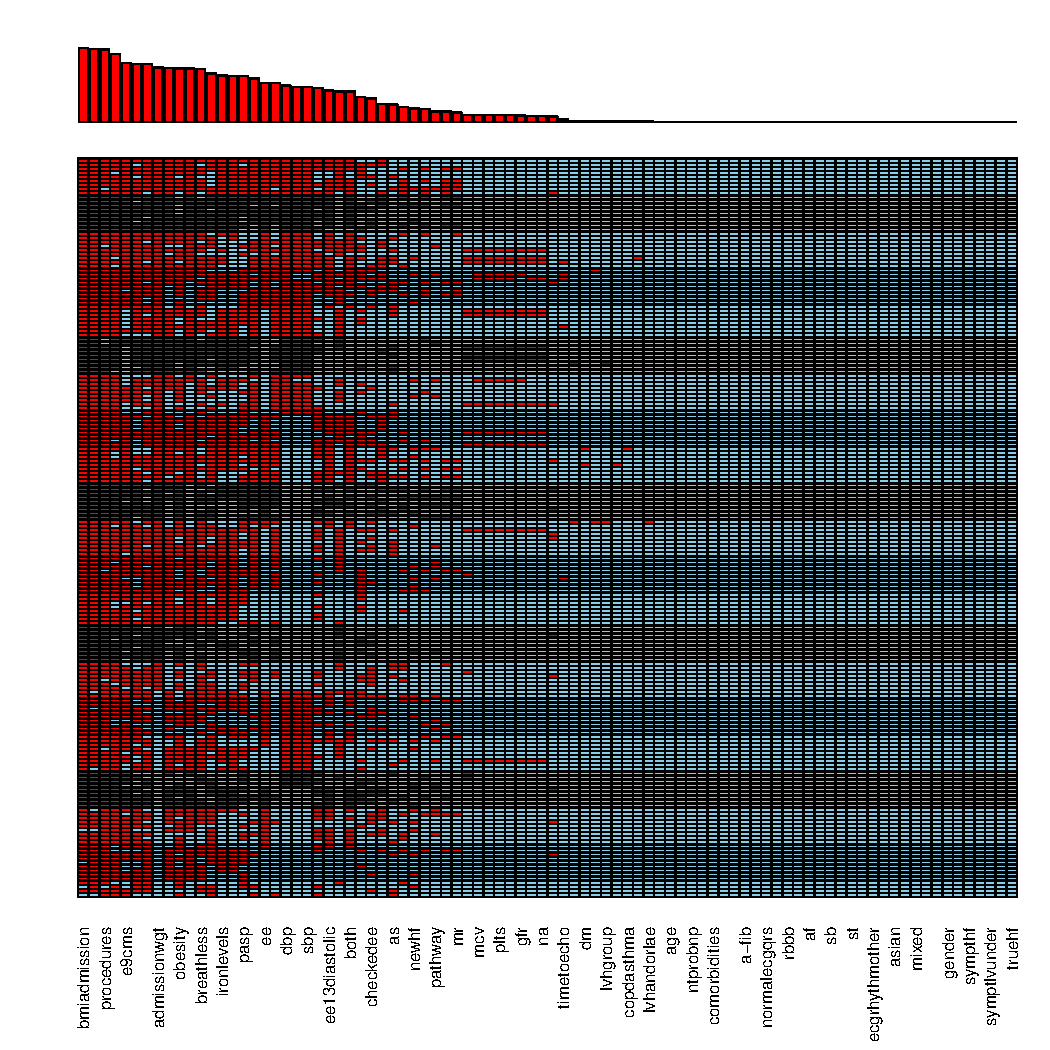
\includegraphics[width=1.1\textwidth]{doc/thesis/images/HFmrEF_miss_dist.pdf}
    \caption[Missing values in HFmrEF data set]{\textit{Missing values in HFmrEF data set. Top:  the amount of missing values in each variable sorted in ascending order. Bottom: plot of the combinations of missing (red) and non-missing (blue) values in the HFmrEF data set.}}
    \label{fig:HFmrEF_missing}
\end{figure}

\chapter{Source Code}
\label{chap:souce_code}

\noindent The following appendix presents all the relevant \texttt{R}-code used in this thesis. We have organized the chapter in accordance with the various steps in the machine learning procedure adopted in this thesis, see figure (\ref{fig:ML_proc_thesis}). We have tried to comment as much of the source code in order to ensure that an eventual re-examination of the results can be as easy and smooth as possible. Inquires about the code can be forwarded to the author on request.

\section{Helper Functions}
\label{sec:helper_func}

\lstinputlisting[language=R]{../../data/data_sets/imputation/_helper_func.R}

\section{Loading Data and Label Extraction}
\label{sec:load_data}

\lstinputlisting[language=R]{../../data/data_sets/raw_data/r_data_sets.R}

\section{Imputation}

\end{document}